% ============================================================
% Cheat sheet, argomento 1: il diagramma delle classi, gli elementi (dispensa, capitolo 7)
% ============================================================
\argomento{Il diagramma delle classi: classi, attributi, operazioni}{Dispensa: capitolo 7}[Classi, attributi, operazioni]

\voce{classe}{Classe}{rettangolo con tre scomparti}
  {\begin{tikzpicture}
     \umlclass[4.2cm]{c}{(0,0)}{Conto}{- intestatario: String\\- saldo: double = 0}{+ deposita(importo: double)\\+ getSaldo(): double}
     \node[ruolo, anchor=west, text=swgray] at ($(c.north east)+(0.05,-0.2)$) {nome};
     \node[ruolo, anchor=west, text=swgray] at ($(c.east)+(0.05,0.12)$) {attributi};
     \node[ruolo, anchor=west, text=swgray] at ($(c.south east)+(0.05,0.32)$) {operazioni};
   \end{tikzpicture}}
  {Il \textbf{nome} è in grassetto, al centro, al \textbf{singolare} (\code{Studente}, non \code{Studenti}). Sotto, gli
   \textbf{attributi} e le \textbf{operazioni}. In Java è una \code{class}: gli attributi sono i campi, le operazioni i
   metodi.}

\voce{soppresse}{Livelli di dettaglio}{regola delle informazioni soppresse}
  {\begin{tikzpicture}
     \node[classe1=1.6cm] (r1) at (0,0) {Rettangolo};
     \umlclass[1.7cm]{r2}{(1.85,-0.12)}{Rettangolo}{altezza\\larghezza}{}
     \umlclass[2.2cm]{r3}{(4.1,-0.35)}{Rettangolo}{altezza: int\\larghezza: int}{getArea(): int}
   \end{tikzpicture}}
  {Tutti e tre sono la \textbf{stessa} classe. Ciò che manca non è assente: è solo \textbf{non mostrato} in quel
   diagramma. Nel modello di dominio bastano nomi e attributi; nel progetto di dettaglio si aggiungono tipi,
   visibilità e operazioni.}

\voce{attributo}{Sintassi di un attributo}{solo il nome è obbligatorio}
  {\uml{\textcolor{ph4}{-} \textcolor{q8}{nome} \textcolor{q5}{[1]}: \textcolor{ph3}{String}\\ = \textcolor{swred}{"Senza titolo"} \{readOnly\}}\par\medskip
   {\footnotesize\color{swgray}\uml{visibilità nome molteplicità: tipo = default \{proprietà\}}}}
  {Un attributo \textbf{privato} di nome \code{nome}, con un solo valore, di tipo \code{String}, che vale all'inizio
   \code{"Senza titolo"} e non si può modificare. In Java:
   \code{private final String nome = "Senza titolo";}. Il tipo è un tipo primitivo o di libreria; se è una classe
   del diagramma, si disegna un'\textbf{associazione} (\vv{tipiattributo}).}

\voce{operazione}{Sintassi di un'operazione}{direzione dei parametri: in, out, inout}
  {\uml{\textcolor{ph4}{+} \textcolor{q8}{preleva}(\textcolor{q5}{in} importo: \textcolor{ph3}{double}):\\ \textcolor{ph3}{boolean} \{query\}}\par\medskip
   {\footnotesize\color{swgray}\uml{visibilità nome(direzione nome: tipo = default, \ldots): tipo \{proprietà\}}}}
  {I parametri si scrivono \code{nome: tipo}, al contrario di Java. La direzione predefinita è \code{in} (in Java i
   parametri sono sempre \code{in}). Il tipo ritornato va dopo i due punti; \code{void} si omette. \code{\{query\}}
   dice che l'operazione non modifica l'oggetto \oltre.}

\voce{visibilita}{Visibilità}{per attributi e operazioni}
  {\begin{tikzpicture}
     \umlclass[3.4cm]{v}{(0,0)}{Esempio}{+ pubblico: int\\\# protetto: int\\- privato: int\\\textasciitilde\ dipackage: int}{}
   \end{tikzpicture}}
  {\begin{tabular}{@{}>{\ttfamily\bfseries}l l >{\ttfamily}l@{}}
     + & tutte le classi & public \\
     \# & le sottoclassi & protected \\
     - & solo la classe & private \\
     \textasciitilde & lo stesso package & \textrm{(nessun modificatore)} \\
   \end{tabular}}

\voce{molteplicita}{Molteplicità}{quanti valori: array e collezioni}
  {\begin{tikzpicture}
     \umlclass[4.3cm]{m}{(0,0)}{Studente}{matricola: String\\secondoNome: String [0..1]\\telefoni: String [1..*]\\voti: int [*]\\ultimiTre: int [3]}{}
   \end{tikzpicture}}
  {\begin{tabular}{@{}>{\ttfamily\bfseries}l l@{}}
     1 & uno e uno solo (\textbf{predefinita}) \\
     0..1 & al più uno (può mancare: \code{null}) \\
     * & quanti si vuole, anche nessuno (\code{0..*}) \\
     1..* & almeno uno \\
     3 \textrm{o} 2..5 & esattamente 3; da 2 a 5 \\
   \end{tabular}}

\voce[88mm]{collezioni}{Ordinati e duplicati}{\{ordered\}, \{nonunique\}: quale collezione Java}
  {\renewcommand{\arraystretch}{1.3}\footnotesize
   \begin{tabular}{@{}r|>{\centering\arraybackslash}p{27mm}|>{\centering\arraybackslash}p{31mm}@{}}
                  & \textbf{senza duplicati} & \textbf{con duplicati} \\ \hline
     \textbf{non ordinati} & \textit{(nessuna proprietà)}\newline \code{Set}, \code{HashSet}
                           & \uml{\{nonunique\}}\newline \textit{nessuna classe Java} \\ \hline
     \textbf{ordinati}     & \uml{\{ordered\}}\newline \code{TreeSet}, \code{LinkedHashSet}
                           & \uml{\{ordered, nonunique\}}\newline \code{List}, \code{ArrayList}, array \\
   \end{tabular}}
  {Per UML gli elementi di una molteplicità sono un \textbf{insieme}: niente ordine, niente duplicati. Le proprietà
   tra graffe lo cambiano. Per una lista di oggetti basta di solito \code{\{ordered\}}; \code{\{nonunique\}} si aggiunge
   quando lo stesso valore può davvero ripetersi, come nei voti (\vv{arrayprimitivi}, \vv{lista}).}

\voce{statico}{Membri statici}{sottolineati}
  {\begin{tikzpicture}
     \umlclass[5.6cm]{s}{(0,0)}{Configurazione}{\underline{- istanza: Configurazione}\\\underline{+ MAX\_UTENTI: int = 100 \{readOnly\}}}{\underline{+ getIstanza(): Configurazione}\\+ leggi(chiave: String): String}
   \end{tikzpicture}}
  {Un campo o un metodo \code{static} appartiene alla classe, non agli oggetti: in UML si \textbf{sottolinea}. Una
   costante \code{static final} è sottolineata e \code{\{readOnly\}}, con il suo valore (\vv{costanti}). È la firma del
   Singleton (\vv{singleton-struttura}).}

\voce{astratta}{Classe e operazioni astratte}{nome in corsivo}
  {\begin{tikzpicture}
     \umlclass[3.6cm]{a}{(0,0)}{\textit{Figura}}{\# colore: String}{+ \textit{area(): double}\\+ descrivi(): String}
     \node[ruolo, anchor=west] at ($(a.north east)+(0.1,-0.25)$) {\{abstract\}};
   \end{tikzpicture}}
  {Classe \code{abstract}: nome in \textit{corsivo} (oppure \code{\{abstract\}} accanto al nome, più leggibile a mano).
   Un metodo \code{abstract} (senza corpo) è in corsivo; gli altri metodi, già implementati, no.}

\voce{interfaccia}{Interfaccia}{stereotipo «interface»}
  {\begin{tikzpicture}
     \umlclass[3.2cm]{i}{(0,0)}{\stereotipo{interface}{Pagabile}}{}{+ paga(importo: double)\\+ getSaldo(): double}
     \node[classe1=1.3cm] (c) at (2.85,-0.1) {Carta};
     \draw[line width=0.7pt] (c.north) -- ++(0,0.45);
     \palla{($(c.north)+(0,0.56)$)}
     \node[ruolo, anchor=west] at ($(c.north)+(0.15,0.56)$) {Pagabile};
   \end{tikzpicture}}
  {Le operazioni sono tutte pubbliche e astratte; di solito non ci sono attributi. In Java è una \code{interface}. A
   destra la forma abbreviata a \textbf{pallina} (\textit{lollipop}): la classe \code{Carta} realizza
   \code{Pagabile} (\vv{lollipop}).}

\voce{enumerazione}{Enumerazione}{stereotipo «enumeration»}
  {\begin{tikzpicture}
     \node[rectangle split, rectangle split parts=2, draw=q9!75!black, fill=yellow!10, line width=0.7pt,
           font=\scriptsize, text width=2.2cm, align=left, inner sep=2.5pt] (e) at (0,0)
           {\centering{\tiny«enumeration»}\\\textbf{Taglia}\par\nodepart{two}PICCOLA\\MEDIA\\GRANDE};
     \umlclass[2.6cm]{m}{(3.3,0)}{Maglietta}{- taglia: Taglia}{}
   \end{tikzpicture}}
  {Un elenco fisso di valori, come l'\code{enum} di Java: nel secondo scomparto i \textbf{letterali}. Si usa come tipo
   degli attributi (\code{taglia: Taglia}) o si collega con una linea di associazione. Con campi e metodi:
   \vv{enumcampi}.}

\voce{costanti}{Costanti e sola lettura}{\{readOnly\}}
  {\begin{tikzpicture}
     \umlclass[4.4cm]{k}{(0,0)}{Ordine}{\underline{+ IVA: double = 0.22 \{readOnly\}}\\- codice: String \{readOnly\}\\- totale: double}{}
   \end{tikzpicture}}
  {Un campo \code{final} non cambia dopo la costruzione: \code{\{readOnly\}}. Se è anche \code{static} è una
   costante della classe, e si sottolinea; il valore si scrive come default (\code{= 0.22}). Per convenzione le
   costanti hanno il nome in maiuscolo.}

\voce{derivato}{Attributo derivato}{la barra: si calcola da altri \oltre}
  {\begin{tikzpicture}
     \umlclass[3.8cm]{d}{(0,0)}{Persona}{- dataNascita: LocalDate\\/ eta: int}{}
   \end{tikzpicture}}
  {Un valore che non si memorizza ma si \textbf{calcola} da altri attributi si scrive con una \code{/} davanti. Nel
   codice di solito non c'è il campo, c'è un metodo: \code{int getEta()} che usa \code{dataNascita}.}

\voce{responsabilita}{Responsabilità}{nei modelli di dominio, al posto dei metodi}
  {\begin{tikzpicture}
     \umlclass[5.4cm]{r}{(0,0)}{Esame}{}{-{}- Gestisce le prenotazioni degli studenti\\-{}- Registra i voti}
   \end{tikzpicture}}
  {Nel modello del \textbf{dominio del problema} non si scrivono metodi (sono un elemento della soluzione), ma
   \textbf{responsabilità}: compiti della classe, preceduti da \code{-{}-}, nello scomparto delle operazioni.}

\voce{nota}{Nota}{commento collegato con una linea tratteggiata}
  {\begin{tikzpicture}
     \node[classe1=1.6cm] (p) at (0,0) {Persona};
     \node[notauml, font=\tiny, text width=2.3cm] (n) at (3.0,0) {deve avere\\almeno 18 anni};
     \draw[tratt] (p.east) -- (n.west);
   \end{tikzpicture}}
  {Testo libero su qualunque elemento di qualunque diagramma: è il \textbf{commento} di UML. Nei pattern contiene
   spesso il codice di un metodo (\code{\{ for all o in observers: o.update() \}}).}

\voce{oggetto}{Oggetto (istanza)}{nome sottolineato \oltre}
  {\begin{tikzpicture}
     \node[rectangle split, rectangle split parts=2, draw=black!75, fill=white, line width=0.7pt,
           font=\scriptsize, text width=3.2cm, align=left, inner sep=2.5pt] (o) at (0,0)
           {\centering\underline{mioConto : Conto}\par\nodepart{two}intestatario = "Anna"\\saldo = 250.0};
   \end{tikzpicture}}
  {Un oggetto si scrive \underline{\code{nome : Classe}} (sottolineato), con i \textbf{valori} dei campi. È la notazione
   dei partecipanti dei diagrammi di sequenza (\underline{\code{:Ordine}}) e dei nodi di deployment
   (\underline{\code{headquarters : TicketServer}}).}
